\setchapterabstract{
}
\chapter{Expected Values and Variances}
\vspace{-1.5cm}

%%%%%%INSERT TOC BELOW 1ST SECTION%%%%%%%%%%%%


{\chaptoc\noindent\begin{minipage}[inner sep=0,outer sep=0]{0.9\linewidth}
    \section{Expected Value of a Linear Transformation}\end{minipage}}

\[
E(aX + b) = aE(X) + b
\]

This property shows that the expectation of a linear transformation of \(X\) follows this simple rule, where \(a\) is a constant multiplier and \(b\) is a constant shift.

However, for non-linear transformations, the expectation does not necessarily follow through the transformation:
\[
E(g(X)) \neq g(E(X))
\]

This is incorrect in general. The only special case where this holds is for a constant function, or where \(g(x)\) is a linear transformation. For instance, \(E(1/X)\) is not \(1/E(X)\).


\section{Expected Value of a Function}

You can find the expected value of a function \( g(X) \) as:

\[
E(Y) = E(g(X))
\]

This can be computed without needing the explicit distribution of \( Y \). The method differs for discrete and continuous random variables:

- For discrete variables: 

\[
E(g(X)) = \sum_i g(x_i) P(x_i)
\]

- For continuous variables: 

\[
E(g(X)) = \int_{-\infty}^{\infty} g(x) f_X(x) dx
\]

\Example{
Expected value of a function with \(P(X = k) = \frac{1}{n}, \quad 1 \leq k \leq n\):
Given X number of trials and \( P(X = k) = \frac{1}{n} \):
\[
E(x) = 1 \cdot \frac{1}{n} \dots + n \frac{1}{n} =  \frac{1}{n} \cdot (1 + 2 + 3) = \frac{n + 1}{2}
\]
}

\Example{
Example: Expected Value of \(X^2\)
For example, given \( X \), the number of trials, and \( P(X = k) = \frac{1}{n}, \quad 1 \leq k \leq n \), the expected value can be computed as:
\[
E(X^2) = \sum_i x_i^2 P(x_i) \quad \text{or} \quad E(X^2) = \int_{-\infty}^{\infty} x^2 f_X(x) dx
\]
}

\section{Variance of a Random Variable}
The variance of a random variable \( X \) is:
\[
\text{Var}(X) = E[(X - E(E))^2] = E[(X - \mu)^2] = E(X^2 - 2\mu X + \mu^2) 
\]
\[
E(X^2) - 2\mu E(X) + \mu^2 = E(X^2) - \mu^2  = E(X^2) - [E(X)]^2
\]

Chebishev Inequality: 
For any R.V. P()
\[
P(|X - E(X)| \geq \eta) \leq \frac{\text{Var}(X)}{\eta^2}, then for \eta = k * \sigma \quad P(|X - E(X)| \geq k\sigma) \leq \frac{1}{k^2}
\]

This shows that variance is the difference between the expected value of \( X^2 \) and the square of the expected value of \( X \).

\section{Variance of a Linear Transformation}
For a linear transformation \( aX + b \), the variance follows the rule:
\[
\text{Var}(aX + b) = a^2 \text{Var}(X)
\]

The constant \( b \) shifts the expected value but does not affect the variance.

\section{example 1}
\[
f_X(x) =
\begin{cases} 
\frac{1}{2\sqrt{x}} & 0 \leq x \leq 1 \\
0 & \text{otherwise} \\
\end{cases}
\]

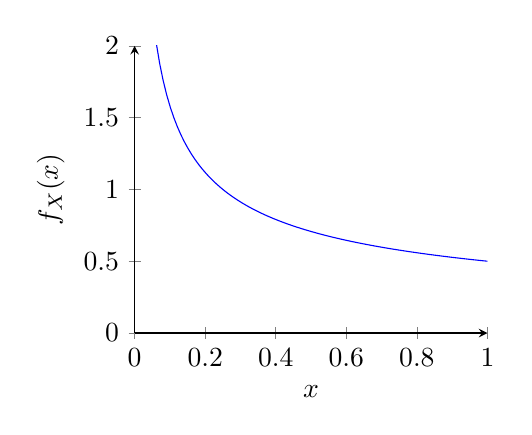
\begin{tikzpicture}
\begin{axis}[
    axis lines = left,
    xlabel = $x$,
    ylabel = {$f_X(x)$},
    ymin=0, ymax=2,
    xmin=0, xmax=1,
    width=0.5\textwidth
]
\addplot [
    domain=0:1, 
    samples=100, 
    color=blue,
]
{1/(2*sqrt(x))};
\end{axis}
\end{tikzpicture}

This is a valid density function because $\pi$ is greater than 0 and the integral from 0 to 1 is 1. 

The cumulative distribution function is: 
\[
F_X(t) =
\begin{cases} 
0 & \text{if } t \leq 0 \\
\sqrt{t} & \text{if } 0 < t < 1 \\
1 & \text{if } t \geq 1 \\
\end{cases}
\]

\begin{tikzpicture}
\begin{axis}[
    axis lines = left,
    xlabel = $t$,
    ylabel = {$F_X(t)$},
    ymin=0, ymax=1.2,
    xmin=0, xmax=1,
    width=0.5\textwidth
]
\addplot [
    domain=0:1, 
    samples=100, 
    color=blue,
]
{sqrt(x)};
\addplot [
    domain=1:2,
    samples=100,
    color=blue,
]
{1};
\end{axis}
\end{tikzpicture}

The expected value is: 
\[
E(x) = \int_0^1 x \cdot f_X(x)dx = \int_0^1 x \cdot \frac{1}{2\sqrt{x}}dx = \int_0^1 \frac{1}{2} \cdot \sqrt{x}dx =[ \frac{1}{2} \cdot \frac{2}{3} \cdot x^{3/2}]_0^1 = \frac{1}{3}
\]
The expected value of $X^2$ is: 
\[
E(X^2) = \int_0^1 x^2 \cdot f_X(x)dx = \int_0^1 x^2 \cdot \frac{1}{2\sqrt{x}}dx = \int_0^1 \frac{1}{2} \cdot x^{3/2}dx = [\frac{1}{2} \cdot \frac{2}{5} \cdot x^{5/2}]_0^1 = \frac{1}{5}
\]
The variance is: 
\[
Var(X) = \frac{1}{5} - (\frac{1}{3})^2 = \frac{4}{45}
\]

\section{Deriving the Marginal Distribution Function of Y}

Given \(X\) and \(Y = g(X)\), if \(g\) is differentiable and invertible (meaning \(y = g(x) \leftrightarrow x = h(y)\)), then 
\[
f_Y(y) = f_X(h(y)) \cdot \left| h'(y) \right|
\]

\section{Example 1}
Given the probability density function of \(X\) as:
\[
f_X(x) =
\begin{cases}
\frac{x-1}{2} & \text{if } 1 \leq x \leq 3 \\
0 & \text{otherwise}
\end{cases}
\]
Then using the indicator function:
\[ f_X(x) = \frac{x-1}{2} \cdot \mathbb{1}_{[1,3]}(x) \]
Let's consider the transformation \(Y = \ln(X)\). It is invertible and differentiable with \(x = h(y) = e^y\). Applying the aforementioned formula, we get:
\[
f_Y(y) = f_X(h(y)) \cdot |h'(y)| = \frac{e^y - 1}{2} \cdot \mathrm{I}_{[\ln(1), \ln(3)]}(y) \cdot e^{y} \cdot |e^{y}| = \frac{e^{y}(e^{y} - 1)}{2} \cdot \mathrm{I}_{[\ln(1), \ln(3)]}(y)
\]
Let's consider the transformation \(Y = X^2\). Generally not invertible, but it is on the support 1-3 such that \(x = h(y) = \sqrt{y}\). 
\[
f_Y(y) = f_X(\sqrt{y}) \cdot \left|\frac{1}{2\sqrt{y}}\right| = \frac{\sqrt{y} - 1}{2} \cdot \mathrm{I}_{[1, 9]}(y) \cdot \sqrt{y} \cdot \frac{1}{2\sqrt{y}} = \frac{\sqrt{y} - 1}{4\sqrt{y}} \cdot \mathrm{I}_{[1, 9]}(y)
\]

\section{Deriving the Cumulative Distribution Function of Y}
\[F_y(t) = P(Y \leq t) = P(g(X) \leq t) - P(g(X) \leq t) = P (X \in At)
\]
\section{Example 2}
\[
F_x(t) = 
\begin{cases}
0 & \text{if } t \leq 1 \\
\frac{(t -1)^2}{4} & \text{if } 1 < t < 3 \\
1 & \text{if } t \geq 3
\end{cases}
\]

If Y = \(X^2\), then the CDF of Y is:
\[
F_Y(t) = P(Y \leq t) = P(X^2 \leq t) = P(X \leq \sqrt{t})
\]
Two cases: 
\[
\begin{cases} 
    0 & \text{if } t \leq 0 \\  P(-\sqrt{t} \leq  x \leq \sqrt{t} ) & \text{if } t > 0 
\end{cases}
\]
\[
F_X(\sqrt{t}) - F_X(-\sqrt{t}) = 
\begin{cases} 
0, & \text{if } \sqrt{t} < 1 \\ 
\left( \frac{\sqrt{t} - 1}{4} \right)^2, & \text{if } 1 \leq \sqrt{t} < 3 \\ 
1, & \text{if } \sqrt{t} \geq 93
\end{cases}
=
\begin{cases}
0, & \text{if } t < 1 \\ 
\left( \frac{\sqrt{t} - 1}{4} \right)^2, & \text{if } 1 < t < 9 \\ 
1, & \text{if } t \geq 9
\end{cases}
\]

\section{Example 3}
\[f_X = \frac{x^2}{18} \cdot \mathbb{1}_{[-3,3]}(x)\]
\[y = x^2: \text{Not invertible, use formula for } F_X.\]
\[
F_X(t) =
\begin{cases}
    0 & \text{if } t < -3 \\
    \frac{t^2 + 27}{54} & \text{if } -3 \leq t \leq 3 \\
    0 & \text{if } t > 3
\end{cases}
\rightarrow F_Y(t) = 
\begin{cases}
    0 & \text{if } t < 0 \\
    * & \text{if } 0 \leq t \leq 9 \\
    1 & \text{if } t > 9
\end{cases}
\]

Clearly, being:
\[ F_Y(t) = P(y \leq t) = P(x^2 \leq t) = P(-\sqrt{t} \leq x \leq \sqrt{t}) = \]
\[F_X(\sqrt{t}) - F_X(-\sqrt{t}) = \frac{\sqrt{t}^2 + 27}{54} - \frac{-\sqrt{t}^2 + 27}{54} = \frac{t}{27} \]
Then:
\[ * = f_Y = \frac{dF_Y}{dt} = \frac{1}{27} \cdot I_{[0,9]}(y) 
\]